\section{Introducción}

Un aspecto muy importante dentro de la disciplina de desarrollo de software, tanto
a nivel de \textit{producto} como de \textit{proceso}, es la \textbf{calidad del
software}.
Esta determina el grado en el que un producto satisface los requerimientos de sus usuarios
tanto internos como externos, y cómo les aporta valor a los mismos.

Se considera que un \textit{modelo de calidad} tiene el objetivo de describir, evaluar y/o
predecir la calidad de un componente \cite{Wagner2013}; y a lo largo de las últimas cuatro
décadas se han propuesto diferentes y diversos modelos \cite{Deissenboeck2009}.
Dentro de este conjunto de diversas propuestas podemos encontrar: modelos taxonómicos, como
lo es la familia de normas ISO/IEC 25000 \cite{iso25000}; modelos basados en métricas como el
índice de mantenibilidad (MI) \cite{Coleman1995}; modelos estocásticos, como los modelos de
crecimiento de confiabilidad (RGMs) \cite{Lyu1996}.

El problema existente con los tipos de modelos nombrados anteriormente viene dado por sus
diferentes propósitos, los cuales fueron clasificados por Deissenbock et al. \cite{Deissenboeck2009}
en tres categorías, y pueden verse en la figura \ref{DAPModels}.
La familia de normas ISO/IEC 25000 tiene como objetivo principal \textit{definir} lo que
corresponde a calidad en un sistema; mientras que un esquema orientado a métricas como MI
pretende \textit{evaluar} el nivel de calidad; mientras que los modelos de crecimiento de
confiabilidad se utilizan para \textit{predecir} la calidad.

\begin{figure}
    \label{DAPModels}
    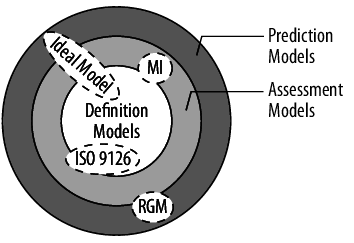
\includegraphics[width=12cm]{quality_metrics/dap_models.png}
    \centering
    \caption{Clasificación de Modelos de Calidad según su propósito.}
\end{figure}

Si bien los diferentes modelos se caracterizan por un objetivo particular, ya sea de
\textit{definición}, \textit{evaluación} o \textit{predicción}, éstos no son independientes,
debido a que es muy difícil evaluar calidad sin una propia definición de la misma, como también
es muy difícil predecir un determinado nivel de calidad sin saber cómo evaluarlo.
Sin embargo, entre los tres tipos planteados, los modelos de evaluación de calidad son considerados
de mucha importancia ya que suelen proveer una guía clara sobre cómo evaluar un sistema y reducir
la brecha entre las métricas de software y los factores de calidad.

Una revisión sistemática de diversos estudios sobre clasificaciones y análisis de los distintos
modelos de calidad, factores o herramientas \cite{Yan2019} establece que los factores de calidad
que son empleados mayoritariamente para determinar la validez de un modelo corresponden a la
mantenibilidad, confiabilidad y eficiencia.
Siendo la mantenibilidad el factor que más se destaca incluso en el conjunto mayormente
considerado, en la siguiente sección se exploran los modelos que definen, miden e incluso
predicen este aspecto en particular.

\section{Mantenibilidad}

\subsection{Definición}

Uno de de los modelos enfocados en la definición de calidad y sus diferentes aspectos
viene establecido por la familia de normas ISO/IEC 25000, 
la cual provee guías para obtener un producto de calidad, mediante la especificación 
de requisitos y características de calidad, así como la evaluación de las mismas.
Esta familia de normas está basada en dos normas anteriores (ISO/IEC 9126
e ISO/IEC 14598), y presenta cinco divisiones, las cuales se enfocan en diferentes
elementos y su proceso.

Particularmente, la norma ISO/IEC 25010, describe el modelo de calidad tanto para el producto
final como para el uso del mismo; definiendo así las características y subcaracterísticas
utilizadas en la evaluación de un elemento, siendo éstas:
\begin{inparaenum}[(1)]
    \item Adecuación funcional,
    \item Eficiencia de desempeño,
    \item Compatibilidad,
    \item Usabilidad,
    \item Fiabilidad,
    \item Seguridad,
    \item Mantenibilidad y
    \item Portabilidad.
\end{inparaenum}
Particularmente, la característica de \textbf{Mantenibilidad} representa la \textit{capacidad del
software para ser modificado de forma eficiente y efectiva, ya sea por motivos correctivos,
evolutivos o perfectivos}.

Así mismo, Mantenibilidad está compuesta por cinco subcaracterísticas:
\begin{inparaenum}[(a)]
    \item Modularidad,
    \item Reusabilidad,
    \item Analizabilidad,
    \item Capacidad para ser modificado \textit{(Modificabilidad)} y
    \item Capacidad para ser probado.
\end{inparaenum}
En el contexto de este trabajo, las subcaracterísticas de mayor interés corresponden
a la \textit{Analizabilidad} y la \textit{Modificabilidad}.
La \textbf{Analizabilidad} está asociada a la facilidad con la que se pueden diagnosticar problemas
o fallas en el software, identificar las partes/componentes de un sistema a modificar, y la
evaluación del impacto generado por los cambios.
Por otro lado, la \textbf{Modificabilidad} viene dada por la capacidad del producto para ser
modificado de forma efectiva y eficiente, sin introducir defectos o afectar la performance.

\subsection{Evaluación}

Así como la familia de normas ISO/IEC 25000 define un conjunto de características y
subcaracterísticas, también provee un listado básico de métricas para su medición.
Este listado no es exhaustivo, ya que se pueden emplear métricas no definidas por el
estándar, siempre y cuando se determine su correlación con alguna de las características
establecidas.
En la tabla \ref{Metrics} se listan las métricas definidas por el estándar, para la \textit{Mantenibilidad}
y sus subcaracterísticas.

\begin{figure}
    \label{Metrics}
    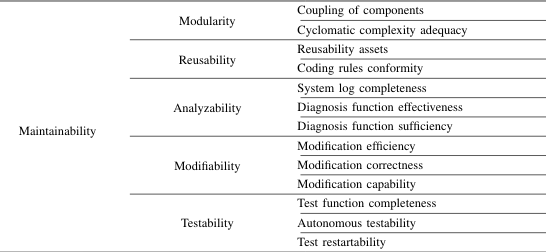
\includegraphics[width=12cm]{quality_metrics/quality_metrics.png}
    \centering
    \caption{Métricas para Mantenibilidad y su subcaracterísticas}
\end{figure}

Sin embargo, este conjunto de normas como otras existentes o anteriores sólo ofrecen una
guía muy abstracta sobre la definición de calidad de software, y no indican cómo lograr
que el software sea de calidad, ni cómo hacer una correcta medición \cite{Relf04}.
Al igual que los primeros modelos escritos a finales de la década de 1970, como los
propuestos por Boehm et al. \cite{Boehm1978} y McCall et al. \cite{McCall1977}, los cuales trataban
de definir la calidad de software como una descomposición jerárquica de características y
subcaracterísticas.

Por lo tanto, la investigación subsiguiente se enfocó principalmente en encontrar maneras de
cuantificar las propiedas definidas por los estudios anteriores.
Los trabajos de Dromey \cite{Dromey1995} y de Bansiya y Davis \cite{Bansiya2002}, son los más 
importantes ya que forman la base sobre la cual se construyeron los modelos más recientes, al 
describir cómo los atributos de alto nivel de calidad pueden medirse a partir de \textit{propiedades
de bajo nivel}, cuantificadas desde \textbf{métricas de software y análisis estático}.

Las contribuciones más significativas en el campo de la \textit{evaluación cuantitativa de la calidad},
basadas en el \textbf{análisis estático de código fuente} vienen dadas por el Modelo de Mantenibilidad 
SIG \cite{Heitlager2007}, junto con Quamoco tool chain \cite{Wagner2012}.

\subsubsection{Modelo de Mantenibilidad SIG}

Este modelo de evaluación de calidad \cite{Heitlager2007} permite determinar la mantenibilidad
de un proyecto de software, donde las características son descompuestas en un
conjunto de subcaracterísticas, y estas últimas en \textit{propiedades}.
Estas propiedades son cuantificables directamente desde el código fuente del producto, utilizando
análisis estático, permitiendo que a partir de estos valores junto con unos determinados umbrales,
cada propiedad reciba un \textit{perfil de calidad}.

Al poder cuantificar estas propiedades y obtener los perfiles, también se pueden agregar,
y de esta manera establecer un puntaje global de calidad del sistema.
Con el fin de mantener la objetividad en los umbrales para la evaluación de propiedades,
estos son obtenidos a través de benchmarking \cite{Alves2010}.

\subsubsection{Quamoco Tool Chain}

Similar al Modelo de Mantenibilidad SIG \cite{Heitlager2007}, Quamoco Tool Chain \cite{Wagner2012}
se basa en propiedades extraídas desde el código fuente a través de análisis estático del mismo,
con la diferencia de que permite a los interesados definir sus propios modelos jerárquicos
de calidad.

Quamoco define un meta-modelo, facilitando la creación de modelos más genéricos, en lugar de
estar restringidos a ciertos atributos de calidad como lo es la mantenibilidad, al introducir
el elementos que permiten cerrar la brecha entre medidas concretas y aspectos abstractos de
calidad.
Toma como base los atributos de calidad definidos en la norma ISO 25010, pero los refina
aplicando 200 factores y 600 mediciones para sistema Java y C\#.

\subsection{Predicción}

\textit{TBD}

\section{Impacto de los Identificadores}

De acuerdo al relevamiento de los diferentes modelos de evaluación de calidad \cite{Yan2019},
las métricas más utilizadas están asociadas a la complejidad, diseño y tamaño del código,
con el fin de obtener mediciones que se correlacionen con los principales factores como la
mantenibilidad, confiabilidad y eficiencia.
Estas métricas suelen extraerse desde el código fuente, incluso considerando los nombres de los
indicadores, los cuales son centrales en el presente estudio.

Si bien el impacto provocado por la baja calidad de los nombres de los indentificadores sobre
la comprensión de programas está razonablemente claro \cite{DeiBenbockPizka05,Lawrie2007,Lawrie2006},
se conoce relativamente poco sobre la influencia que podría ejercer la calidad de los nombres
sobre la calidad total del código fuente \cite{ButlerWemelingerYu10}.
Existen métricas respecto a la \textit{legibilidad} del código, derivadas de varios aspectos como el
número de paréntesis, tamaño de línea, cantidad de espacios en blanco, así como también del
número, frecuencia y longitud de los identificadores \cite{Buse2008}.
Otros estudios propusieron un conjunto de guías de estilo para el nombrado
de identificadores, independiente del lenguaje, para validar su aceptación empírica entre los
programadores \cite{Relf2005}; e incluso utilizar la gramática y otras falencias como pistas para
analizar nombres que puedan ser reescritos \cite{Abebe2009}.
La particularidad de los diferentes estudios comentados anteriormente recae en que
en todos ellos se ignora el contenido semántico de los nombres de los indicadores.

Dado que algunos autores consideran que la elección del \textbf{nombre de un identificador},
especialmente en sistemas de gran tamaño, tiene el potencial de impactar positivamente en el 
nivel de calidad de un sistema \cite{Relf04}, deberían emplearse métricas que consideren este aspecto
al momento de su evaluación.
Además aprovechar la extracción desde el código fuente a través de \textit{análisis estático},
ya que permite \textbf{heurísticas de bajo costo que para identificar regiones del código fuente 
potencialmente problemáticas} \cite{ButlerWemelingerYu10}.
